% =====================================================================
% STEP 1 — THE DISCLOSURE ECOSYSTEM  (rewrite v2, per Ruben's comments)
% Scope: this chapter is ONLY the construction of the necessity-domain
% matrix (screening + the classifying framework) and simple counts +
% the matrix figure. All scoring (what each instrument demands topic by
% topic, opt-in mechanics, sparse-matrix, narrow-law/broad-cascade) moves
% to Steps 3-4 (Ch 7).
% Counts verified against Necessity_Domain_Matrix_v8.xlsx.
%   Chapter presents the FULL landscape (all 49 catalogued); winnowing to the
%   30 scored is deferred to Steps 3-4 (Ch 7), per Ruben.
%   Full-landscape (VSME=Customer): Tiers 19/10/11/9; Domain 19 seafood / 30 general;
%   Source Regulator 19, Customer 14, Investor 6, Industry/NGO 10.  Scored subset = 30.
% =====================================================================

\section{5. The disclosure ecosystem}\label{angle1-ecosystem}

The first step scans the \emph{ecosystem}: it establishes which sustainability
instruments act on a European seafood-processing SME, and classifies each by how
obligatory it is and which stakeholder drives it. In doing so it constructs the
first component of the study's central instrument - the demand matrix - by
fixing and ordering its columns. This chapter does not yet ask \emph{what} each
instrument demands, topic by topic; that scoring, and the convergence it reveals,
is the work of Chapter~7. Here the question is prior and structural, and it is the thesis's first: who asks, and
how bindingly? This is Step~1 of the methodology set out in
Figure~\ref{fig:methodology-overview}.

\subsection{5.1 Constructing the necessity--domain
map}\label{ecosystem-construction}

\textbf{Identifying the instruments.} The instrument set was assembled in three
steps. First, candidate instruments were identified from two complementary
sources: the sustainability reports of the six large seafood processors that form
this study's cohort (Chapter~6), which show the regulations, certifications and
frameworks that leading firms in the sector actually respond to; and a structured
scan of EU sustainability law and the principal voluntary standards, ratings and
initiatives active in the sector. Second, each candidate was screened against two
inclusion gates: that it bears on an environmental, social or governance matter
(excluding purely fiscal, customs and data-protection law), and that it places a
binding obligation on the \emph{organisation itself} - a disclosure,
due-diligence, certification or market-access requirement - rather than merely
binding Member States or granting an individual employee an entitlement. Third,
the classification was built against how the demands are experienced in practice
rather than against formal legal status alone. Industry contacts at Seafood Europe
were consulted on the necessity ranking while it was being drawn up, and the
completed classification has been submitted to the cohort firms for review
(Chapter~4, \nameref{framework-validation-strategy}).

\textbf{A status for each instrument.} The catalogue deliberately keeps the
\emph{whole} field in view: every instrument that acts on the sector is placed in
the map, whether or not it ultimately enters the scored analysis. Each therefore
carries a status alongside its tier, domain, source and locus - the four
classifying attributes introduced below. An instrument is \emph{scored}; held out
as the CSRD/ESRS \emph{baseline} reference; set aside as \emph{context}, binding
Member States rather than the processor, as the Common Fisheries Policy does; or
\emph{excluded} for failing a screening gate, as a purely fiscal law does, or a
benchmark that rates other schemes rather than demanding anything of the
processor.

\textbf{The necessity axis: four tiers.} The framework's spine ranks each
instrument by how imperative it is from the SME's own perspective, on a gradient
of obligation that runs from \emph{coercive}, legally enforced requirements at the
base to \emph{normative}, voluntary commitments at the top - the institutional
gradient developed in Chapter~3 (DiMaggio \& Powell, 1983; Suchman, 1995). The
four tiers make it operational, each a point on that gradient:

\begin{itemize}
\item \textbf{Tier~1 - legal licence to operate.} Binding law, without which
the firm cannot lawfully trade: the IUU and Fisheries Control Regulations,
packaging law, occupational-safety law - coercive obligation in its purest form.

\item \textbf{Tier~2 - market licence to operate.} Legally optional but
commercially non-negotiable: a recognised certification or social audit - MSC, ASC, SMETA and EcoVadis are the most common examples in this sector,
not an exhaustive list - without which a major retail or foodservice
customer will not list a supplier. US Foods, for instance, requires any
GSSI-benchmarked certification (MSC or BAP are given only as examples) for
its top supplier tier and reserves the right to end a supplier relationship
over unresolved non-compliance (US Foods Holding Corp., 2025); several major
retailers make MSC or ASC specifically a sourcing-policy condition (Blank,
2025). The obligation is enforced by the market rather than the state, and
which specific scheme satisfies it varies by buyer and species.

\item \textbf{Tier~3 - competitive expectation.} Increasingly normalised
reporting frameworks whose absence is a competitive disadvantage - the VSME,
GRI, and the value-chain disclosures cascaded from customers under CSRD. This is
the mimetic-normative middle, where firms adopt what peers and buyers expect.

\item \textbf{Tier~4 - strategic differentiation.} Genuinely voluntary
commitments that signal leadership (SBTi, the UN Global Compact, TNFD). Adoption
is elective and reputational.
\end{itemize}

The tiers rank the \emph{instruments} by how binding each is; they do not by
themselves say which \emph{topics} a firm should build first. A firm that answers
only the binding tiers as each demand lands is reactive; the proactive move
(Sharma \& Vredenburg, 1998; Torugsa et al., 2013; the distinction developed in
Chapter~3) is to build, ahead of demand, the shared datapoints that recur across
many instruments regardless of tier, determined instead by how far demand
\emph{converges} across the ecosystem, how many stakeholder channels ask for a
topic, not by tier position.

\textbf{The domain axis.} Cutting across the tiers, the domain axis separates
\emph{seafood-sector-specific} instruments (the fisheries and aquaculture
regulations and certifications, and the GDST traceability standard) from
\emph{general corporate-sustainability} instruments that apply to the processor as
an enterprise like any other (climate, packaging, labour and governance law and
the cross-sector reporting frameworks).

\textbf{Two attributes: source and obligation locus.} Each in-scope instrument
carries two further tags. Its \emph{source} is the stakeholder whose demand the
processor actually answers, assigned by a single test - does the instrument
legally bind the processor? Where it does, the source is the \emph{regulator} (the
Fisheries Control Regulation binds the processor directly). Where it does not, the
source is the stakeholder that transmits the demand: a retailer-required
certification such as MSC codes to \emph{customer}; a capital-market standard such
as SFDR to \emph{investor}; an NGO-led framework such as GDST to
\emph{industry/NGO}. This test deliberately reassigns instruments whose nominal
issuer is a regulator to the channel through which a sub-threshold SME actually
meets them: CSRD and CSDDD, written for large undertakings, reach the small
processor not as law it must obey but as data its large customers must extract
from it, and so code to \emph{customer}. The same reasoning codes the VSME to the
customer channel: although a voluntary standard, in practice a small seafood
processor adopts it to answer a large customer's value-chain request rather than
to address capital markets. This does partly double-count the ESRS content that
also reaches the firm through CSDDD - a limitation accepted here because, for
seafood processors specifically, that demand genuinely arrives through the
customer channel.

The \emph{obligation locus} records, separately from source, whether the
processor is itself the bound party: \emph{direct} where the processor is the
obligated, certified or reporting entity (a processor holding MSC
chain-of-custody certification, which it maintains and is audited against);
\emph{indirect} where the obligation sits elsewhere and reaches the processor
through a buyer's demand or its own disclosure duty (CSDDD, which binds the large
customer and arrives as a value-chain questionnaire); and \emph{context} where
the instrument binds a Member State or another actor with no mechanism that
transmits an obligation to the processor at all (the Common Fisheries Policy).
Holding source and locus apart prevents the common error of reading the legally
bound party off the identity of the actor who actually applies the pressure.

\textbf{Two caveats on the map.} First, the instrument set is calibrated to
leading firms: it was screened from the reports of six large processors, so it
captures what mature, well-resourced firms respond to. It may therefore both
include instruments a small SME does not yet face and understate informal or
local demands it does. Second, necessity is profile-dependent. The tiering
assumes the modelled SME - a business-to-business supplier selling to large EU
retailers and exporting - for which retailer certifications are a genuine
market licence; a firm selling locally or direct to consumers would re-tier
several instruments.

\subsection{5.2 The instrument landscape}\label{ecosystem-landscape}

The catalogue comprises \textbf{49 instruments}
(Figure~\ref{fig:necessity-domain}) - the full field acting on a European
seafood processor. Read as counts, the landscape has three features.

By \emph{necessity tier}, it is weighted toward the binding base: 19 instruments
sit at Tier~1 (legal licence to operate), 10 at Tier~2 (market licence), 11 at
Tier~3 (competitive expectation) and 9 at Tier~4 (strategic differentiation). The
mandatory legal floor is the single largest block.

By \emph{stakeholder source}, regulators account for 19 instruments and customers
for 14 - together two-thirds of the field - while investors (6) and industry
or NGO initiatives (10) make up the remainder. What a small processor faces is
thus overwhelmingly a regulator-and-customer affair.

By \emph{domain}, 19 instruments are seafood-sector-specific - the fisheries and
aquaculture regulations and certifications together with the GDST traceability
standard - and 30 are general corporate-sustainability instruments. Most of what
acts on a seafood processor is not peculiar to seafood at all.

Of these 49, thirty enter the scored demand matrix in Chapter~7; the remainder
are held out as the CSRD/ESRS baseline, set aside as context because they bind
Member States rather than the processor, or excluded for failing a screening
gate. Every instrument named here is defined in full - the organisation behind
it, its legal reference, current status and official source - in the
\nameref{app:glossary}.

\begin{figure}[ht]
\centering
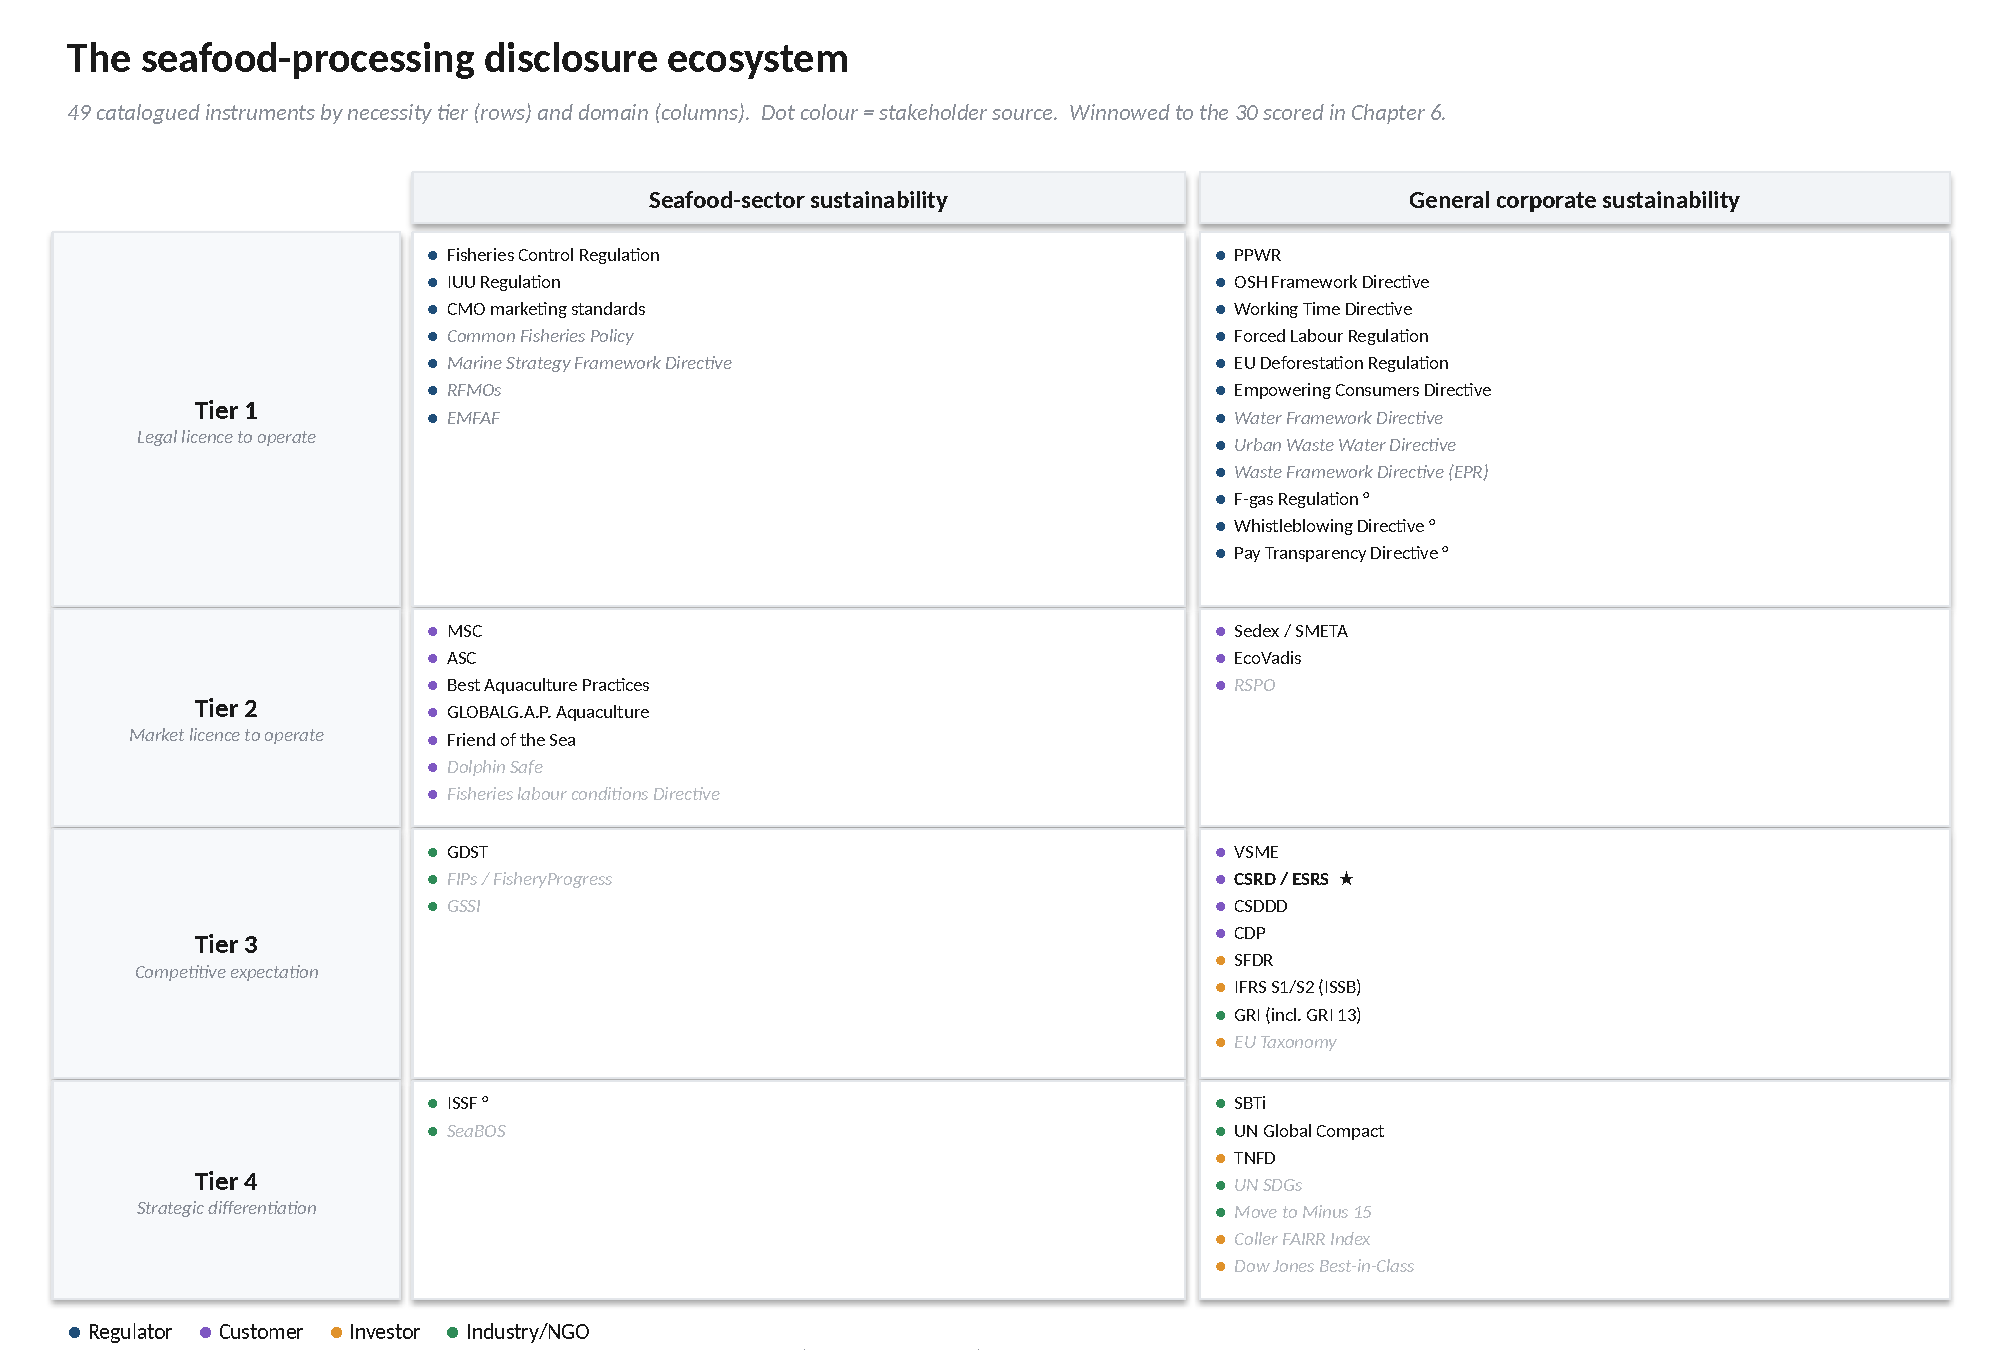
\includegraphics[width=\linewidth]{necessity_domain_matrix.pdf}
\caption{The seafood-processing disclosure ecosystem: all 49 catalogued
instruments arranged by necessity tier (rows) and domain (columns). Dot colour
marks the stakeholder source; text style marks status - normal = scored,
``\,\textdegree\,'' = firm-profile opt-in, $\star$~= the CSRD/ESRS baseline, grey
italic = context (binds Member States, not the processor), pale = excluded. The
winnowing to the 30 scored instruments is set out in Chapter~7. A full reference
entry for each instrument - the body behind it, its legal reference, status and
official source - is given in the \nameref{app:glossary}.}
\label{fig:necessity-domain}
\end{figure}

This map fixes the columns of the demand matrix: who asks, and how bindingly. What
each instrument actually demands, topic by topic, and where those demands
converge into build-first priorities, is taken up in Chapter~7. First, however,
Chapter~6 turns to the rows - establishing, from the disclosures of the sector's
most advanced reporters, what a mature seafood firm actually reports.
